\section{Mise en place et exploitation du laboratoire de tests}

\subsection{Objectifs du laboratoire}

Le laboratoire de tests a été mis en place afin de reproduire une
infrastructure Check Point représentative d’un environnement de
production. Il permet d’expérimenter le déploiement et
l’administration des différents composants de sécurité tout en
analysant leur comportement dans plusieurs scénarios
d’exploitation.

Plus précisément, ce laboratoire vise à :

\begin{itemize}
    \item étudier l’architecture Check Point et ses mécanismes de gestion ;
    \item expérimenter l’architecture \textit{Multi-Domain Manager} ;
    \item analyser le processus de déploiement des politiques de sécurité ;
    \item observer les mécanismes de haute disponibilité via le clustering.
\end{itemize}

L’infrastructure a été déployée dans un environnement virtualisé
afin de simuler plusieurs domaines de sécurité tout en conservant
une architecture proche de celle rencontrée dans des
environnements réels.

%------------------------------------------------

\subsection{Architecture générale du laboratoire}

Le laboratoire repose sur une architecture Check Point classique
composée de trois éléments principaux : une interface
d’administration, un serveur de management et une ou plusieurs
passerelles de sécurité. Ces composants interagissent selon un
modèle hiérarchique dans lequel les politiques de sécurité sont
définies par l’administrateur, centralisées sur un serveur de
management puis déployées vers les passerelles chargées
d’inspecter le trafic réseau.

La figure~\ref{fig:archi_lab} illustre l’organisation générale de
cette architecture. Les différents composants y sont numérotés
afin de faciliter leur identification dans les descriptions
suivantes.

\begin{figure}[H]
    \centering
    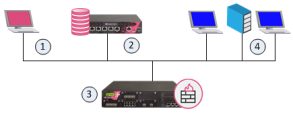
\includegraphics[width=0.75\textwidth]{assets/archi_ckp.png}
    \caption{Architecture générale du laboratoire}
    \label{fig:archi_lab}
\end{figure}

\paragraph{SmartConsole (1).}

La \textbf{SmartConsole} constitue l’interface graphique
d’administration de l’environnement Check Point. Elle permet à
l’administrateur de définir les politiques de sécurité, de gérer
les objets réseau et d’analyser les journaux d’événements.

La SmartConsole ne stocke aucune configuration localement. Toutes
les actions effectuées par l’administrateur sont transmises au
serveur de management via un canal sécurisé appelé
\textit{Secure Internal Communication} (SIC).

\paragraph{Serveur de management (2).}

Le serveur de management constitue le cœur du système de gestion.
Il centralise l’ensemble des politiques de sécurité, la base
d’objets réseau ainsi que les journaux d’événements.

Dans l’architecture du laboratoire, ce rôle est assuré par un
\textbf{Multi-Domain Manager} (MDM). Ce composant permet
d’administrer plusieurs domaines de sécurité indépendants à
partir d’une plateforme unique.

Les politiques de sécurité définies dans la SmartConsole sont
compilées par le serveur de management puis déployées vers les
passerelles via l’opération \textit{Install Policy}.

\paragraph{Security Gateway (3).}

La \textbf{Security Gateway} est l’équipement chargé d’inspecter
le trafic réseau. Positionnée en coupure sur le réseau, elle
applique les politiques de sécurité reçues depuis le serveur de
management et analyse les flux en temps réel.

\paragraph{Environnement à protéger (4).}

L’environnement à protéger représente l’ensemble des ressources
internes du réseau : postes de travail, serveurs et services
applicatifs. Dans le cadre du laboratoire, cet environnement
simule un périmètre client afin d’observer le comportement des
passerelles de sécurité dans des conditions proches d’un
environnement réel.

%------------------------------------------------

\subsection{Architecture Multi-Domain Manager}

Afin de reproduire un environnement multi-client, le laboratoire
s’appuie sur l’architecture \textbf{Multi-Domain Manager} (MDM)
proposée par Check Point \cite{checkpoint_mds_r8030}.

Le Multi-Domain Manager constitue le serveur central de
management. Il permet d’administrer simultanément plusieurs
domaines de sécurité indépendants à partir d’une plateforme
unique. L’administrateur s’y connecte via la SmartConsole afin
de superviser les différents domaines, gérer les objets globaux,
administrer les comptes utilisateurs et consulter les journaux
centralisés.

Cette architecture permet de gérer plusieurs domaines de sécurité
indépendants depuis un point d’administration centralisé. Chaque
domaine dispose de ses propres politiques de sécurité, de ses
objets réseau et de ses passerelles, tout en restant isolé des
autres domaines.

La figure~\ref{fig:mds_overview} illustre l’organisation générale
d’un déploiement multi-domaine.

\begin{figure}[H]
    \centering
    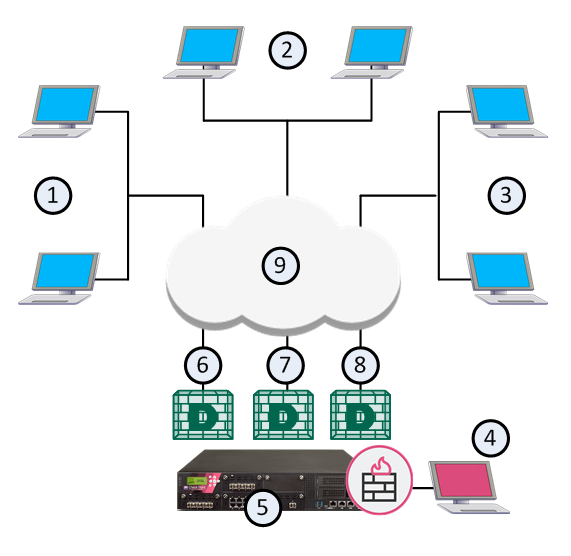
\includegraphics[width=0.75\textwidth]{assets/mds_overview.png}
    \caption{Architecture générale du laboratoire}
    \label{fig:mds_overview}
\end{figure}


\subsubsection{Customer Management Add-on / Domain Management Server}

Au sein du Multi-Domain Manager, chaque domaine est administré
par un \textbf{Domain Management Server} (DMS), historiquement
appelé \textbf{Customer Management Add-on} (CMA).

Chaque DMS constitue un serveur de management autonome,
équivalent à un Security Management Server dans une architecture
mono-domaine.

Il administre de manière indépendante :

\begin{itemize}
    \item les politiques de sécurité et les règles NAT ;
    \item les objets réseau du domaine ;
    \item les Security Gateways associées ;
    \item les journaux et paramètres propres au domaine.
\end{itemize}

Cette séparation garantit qu’un administrateur d’un domaine ne
peut accéder ni aux données ni aux politiques d’un autre domaine,
ce qui est particulièrement important dans les environnements
multi-clients.

%------------------------------------------------

\subsection{Déploiement des passerelles de sécurité}

Les politiques définies dans les différents Domain Management
Servers sont déployées vers les passerelles de sécurité
associées. Ces équipements constituent les éléments chargés
d’appliquer effectivement les règles de sécurité sur le trafic
réseau.

\subsubsection{Security Gateway}

Une \textbf{Security Gateway} est un équipement positionné en
coupure sur le réseau qui reçoit la politique compilée depuis
son serveur de management. Elle inspecte ensuite le trafic en
temps réel afin de déterminer si les communications doivent être
autorisées ou bloquées.

Les journaux générés lors de l'inspection du trafic sont
ensuite envoyés vers le serveur de management afin d’être
analysés dans la SmartConsole.

\subsubsection{Déploiement en cluster}

Afin de garantir la continuité de service, les Security Gateways
peuvent être déployées en \textbf{cluster} grâce à la technologie
\textbf{ClusterXL} de Check Point.

Un cluster regroupe plusieurs passerelles physiques qui partagent
une adresse IP virtuelle et fonctionnent comme un seul
équipement du point de vue du réseau et du serveur de management.

Dans un cluster classique à deux membres, les passerelles peuvent
se trouver dans les états suivants :

\begin{itemize}
    \item \textbf{Active} : la passerelle traite le trafic réseau ;
    \item \textbf{Standby} : la passerelle est synchronisée et prête
    à prendre le relais ;
    \item \textbf{Down} : la passerelle n’est plus opérationnelle.
\end{itemize}

En fonctionnement normal, seul le membre \textit{Active} traite le
trafic. En cas de défaillance  (\textit{failover}), le membre \textit{Standby} prend
automatiquement le relais, garantissant la
continuité du service sans interruption.

La figure~\ref{fig:cluster_states} illustre les états possibles d'un
cluster à deux membres.
 
\begin{figure}[H]
    \centering
    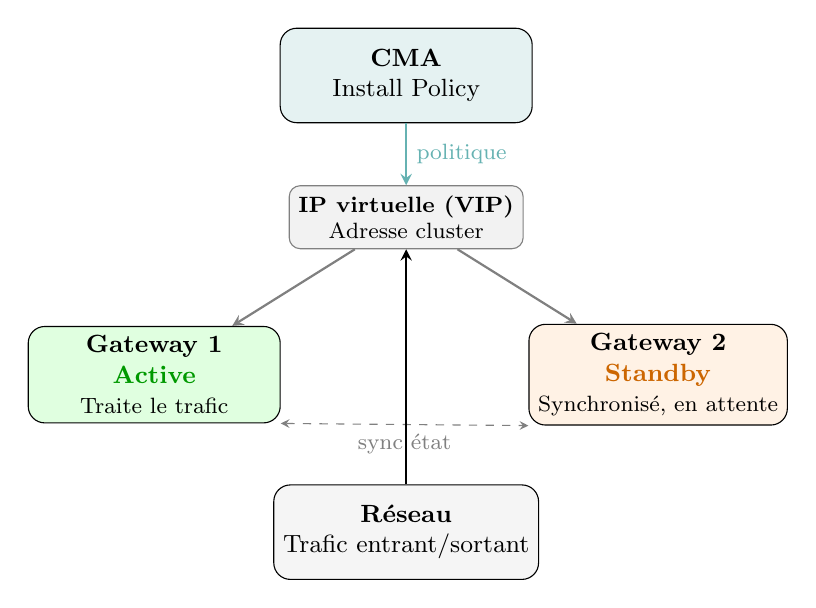
\begin{tikzpicture}[
        gwbox/.style  = {rectangle, draw, rounded corners=6pt,
                         minimum width=3.2cm, minimum height=1.2cm,
                         font=\small, align=center},
        vipbox/.style = {rectangle, draw=black!50, rounded corners=4pt,
                         minimum width=2.4cm, minimum height=0.8cm,
                         font=\footnotesize, align=center, fill=gray!10},
        arr/.style    = {->, >=stealth, thick},
        lbl/.style    = {font=\footnotesize}
    ]
        \node[vipbox] (vip) at (0, 3.2)
            {\textbf{IP virtuelle (VIP)}\\Adresse cluster};
        \node[gwbox, fill=teal!10] (cma) at (0, 5.0)
            {\textbf{CMA}\\Install Policy};
        \node[gwbox, fill=green!12] (gwa) at (-3.2, 1.2)
            {\textbf{Gateway 1}\\
             \textcolor{green!60!black}{\textbf{Active}}\\
             {\footnotesize Traite le trafic}};
        \node[gwbox, fill=orange!10] (gwb) at (3.2, 1.2)
            {\textbf{Gateway 2}\\
             \textcolor{orange!80!black}{\textbf{Standby}}\\
             {\footnotesize Synchronisé, en attente}};
        \node[gwbox, fill=gray!8] (net) at (0, -0.8)
            {\textbf{Réseau}\\Trafic entrant/sortant};
 
        \draw[arr, teal!60]  (cma)  -- node[right, lbl]{politique} (vip);
        \draw[arr, black!50] (vip)  -- (gwa);
        \draw[arr, black!50] (vip)  -- (gwb);
        \draw[<->, >=stealth, dashed, gray]
            (gwa.south east) -- node[below, lbl]{sync état} (gwb.south west);
        \draw[arr] (net.north) -- (vip.south);
    \end{tikzpicture}
    \caption{Security Gateway en cluster~: états Active et Standby}
    \label{fig:cluster_states}
\end{figure}
